\documentclass[11pt]{article}
\usepackage{mathtools}
\usepackage{epsfig,psfrag}
\usepackage{listings}
\usepackage{color}
\usepackage{amssymb}
\usepackage[T1]{fontenc}
\usepackage{lipsum} % Package to generate dummy text throughout this template
\usepackage[brazil]{babel}
\usepackage[sc]{mathpazo} % Use the Palatino font
\usepackage[T1]{fontenc} % Use 8-bit encoding that has 256 glyphs
\usepackage[utf8]{inputenc}
\linespread{1.05} % Line spacing - Palatino needs more space between lines
\usepackage{microtype} % Slightly tweak font spacing for aesthetics
\usepackage{algpseudocode}
\usepackage{algorithmicx}

\usepackage[hmarginratio=1:1,top=32mm,columnsep=20pt]{geometry} % Document margins
\usepackage{multicol} % Used for the two-column layout of the document
\usepackage[hang, small,labelfont=bf,up,textfont=it,up]{caption} % Custom captions under/above floats in tables or figures
\usepackage{booktabs} % Horizontal rules in tables
\usepackage{float} % Required for tables and figures in the multi-column environment - they need to be placed in specific locations with the [H] (e.g. \begin{table}[H])
\usepackage{hyperref} % For hyperlinks in the PDF

\usepackage{lettrine} % The lettrine is the first enlarged letter at the beginning of the text
\usepackage{paralist} % Used for the compactitem environment which makes bullet points with less space between them

\usepackage{abstract} % Allows abstract customization
\renewcommand{\abstractnamefont}{\normalfont\bfseries} % Set the "Abstract" text to bold
\renewcommand{\abstracttextfont}{\normalfont\small\itshape} % Set the abstract itself to small italic text

\usepackage{titlesec} % Allows customization of titles
\selectlanguage{brazil}

\usepackage{fancyhdr} % Headers and footers
\pagestyle{fancy} % All pages have headers and footers
\fancyhead{} % Blank out the default header
\fancyfoot{} % Blank out the default footer
\fancyhead[C]{{\vspace{-3cm}{\hspace{-4cm}\mbox{\begin{minipage}{1.5cm} \epsfxsize=2cm
\centerline{\epsffile{unimontes.eps}}
\end{minipage}}}{\hspace{.6cm} Projeto e Análise de Algoritmos $\bullet$ 2015}} 
} % Custom header text
\fancyfoot[RO,LE]{\thepage} % Custom footer text




%----------------------------------------------------------------------------------------
%    TITLE SECTION
%----------------------------------------------------------------------------------------

\title{\vspace{.5cm}\fontsize{24pt}{10pt}\selectfont\textbf{\sc Lista de Exercícios - Análise de algoritmos}} % Article title

\author{
\large
\textsc{Herberth Amaral}\\[2mm] % Your name
\normalsize Departamento de Ciência da Computação \\
\normalsize Universidade Estadual de Montes Claros \\
\normalsize \href{mailto:herberthamaral@gmail.com}{herberthamaral@gmail.com} % Your email address
\vspace{-5mm}
}
\date{\today}

%----------------------------------------------------------------------------------------

\begin{document}

\maketitle % Insert title

\thispagestyle{fancy} % All pages have headers and footers

%----------------------------------------------------------------------------------------
%    ABSTRACT
%----------------------------------------------------------------------------------------
%\begin{abstract}
%\noindent O presente trabalho analisa o uso de redes neurais artificiais do
%tipo perceptron de múltiplas camadas para fazer classificação de dados de
%comparação de registros, a fim de categorizá-los como registros correspondentes
%ou não-correspondentes, em um processo conhecido como record linkage.  A base
%de dados contém os resultados de comparação de dados demográficos provenientes
%do registro epidemiológico de câncer do estado alemão de Rhine-Westphalia \cite{west}.
%Os resultados mostram que a rede neural usada neste trabalho conseguiu
%classificar os registros satisfatoriamente.
%
% 
%\end{abstract}

\newpage

\section*{Exercícios}

\begin{enumerate}
    \item A complexidade é dada pelo número de arestas: $O(|E|)$
    \item Quer dizer que o algoritmo \textit{find} executa um número de
operações proporcional a $n log(n)$, em que $n$ é o tamanho da entrada do
algoritmo. De fato, como a função de Ackermann cresce muito rapidamente (mesmo
para valores muito pequenos, como 4,3), o seu inverso é usado para denotar
funções que crescem muito devagar.
    \item A principal diferença entre o QuickSort e o MergeSort é a
complexidade no pior caso. No MergeSort é $O(nlogn)$ e no QuickSort é $O(n^2)$,
entretanto é raro o QuickSort atingir o pior caso. Segue abaixo uma
implementação em Python do QuickSort: \hfill \\
    \lstinputlisting[language=Python]{quicksort.py}
    A seguir, uma implementação do MergeSort em Python
    \lstinputlisting[language=Python]{mergesort.py}
    \item Os dois algoritmos tem a mesma complexidade de tempo: $O(|V|+|E|)$,
porém o algoritmo de Tarjan possui uma iteração a menos e, por isso, na
prática, tende a ser mais rápido.
    \item Os dois algoritmos podem apresentar complexidade $O(|E|log|V|)$. Essa
complexidade pode variar de acordo com o uso de algoritmos de ordenação e
estruturas de dados utilizadas para representar o grafo.
    \item Sim, há o algoritmo de Thorup (\cite{thorup}) que possui complexidade linear, ou $O(n)$. O algoritmo de Dijkstra possui complexidade proporcional a $O(|E| + |V|log|V|)$.
    \item A complexidade dos algoritmos do heap binário são:
        \begin{enumerate}
            \item Busca: $O(n)$
            \item Inserção: $O(logn)$
            \item Exclusão: $O(logn)$
        \end{enumerate}    
    \item \hfill \\
        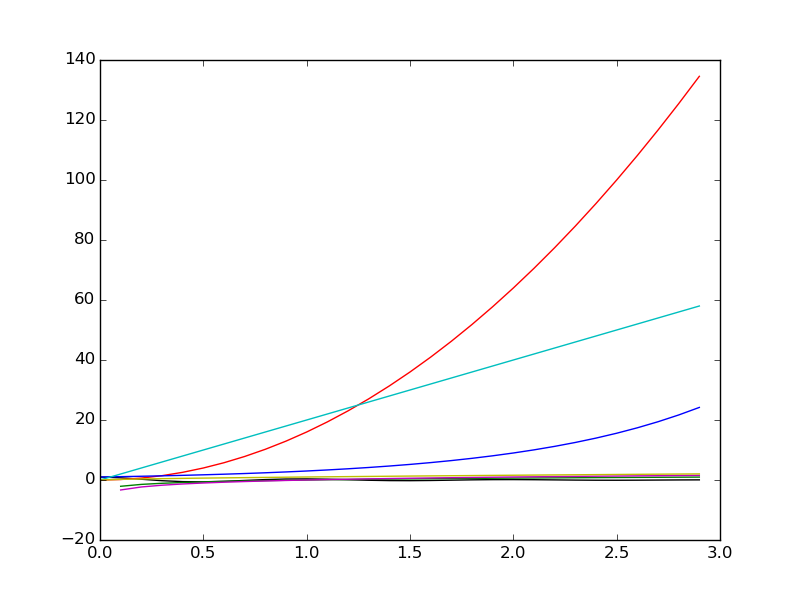
\includegraphics[scale=0.5]{plot.png}
    \item A soma de vetores em tempo $O(logn)$ não é possível, pois é necessário fazer uma soma par-a-par de todos os elementos do subvetor. Portanto, esse tipo de operação é $\Omega(n)$. Entretanto, a primeira função encontra-se abaixo: \hfill \\
        \lstinputlisting[language=Python]{soma.py}
    \item 
        \begin{enumerate}
            \item Realiza a soma dos $a$ primeiros números naturais;
            \item Como a função está escrita no formato \textit{tail-recursive}, é possível reescreve-la para um formato iterativo de forma a facilitar os cálculos: \hfill \\
                \lstinputlisting[language=C]{x.c}
                Desta forma é fácil verificar que X é da ordem de $2n + 2$.
            \item Feito no item anterior;
            \item As duas funções são equivalentes em termos de complexidade
assintótica.  No entanto, na prática, caso o compilador não tenha otimização de
\textit{tail-call}, a implementação iterativa é mais eficiente.
        \end{enumerate}
    \item A partir de $n=3$.
    \item 
        \begin{enumerate}
            \item Afirmativa verdadeira. $2^{n+1}$ domina assintoticamente $2^n$;
            \item Afirmativa falsa. $2^{2n}$ domina assintoticamente $2^n$, pois não há uma constante que multiplicada por $2^{n}$ seja $>=2^{n+1}$;
            \item Afirmativa falsa. Contra-exemplo: $ f(n) = O(n), g(n) = O(1) \rightarrow f(n) + g(n) = O(n)$.
        \end{enumerate}
    \item $O(n*i*j)$
    \item A pizza ganha dois novos pedaços a cada corte. Portanto $P(n) = 2n$.
    \item Prova por indução. Assumindo que o algoritmo analisado considera
potenciação como uma série de multiplicações e que o algoritmo considere uma
mútiplicação como uma série de somas, $n = 2 \rightarrow \Sigma_{i=0}^2 3^i = 3.3 = (3+3+3) = \Sigma_{j=0}^{3^1} 3$. Para 
$n = 3 \rightarrow \Sigma_{i=0}^3 3^i = 3.3.3 = (3+3+3+3+3+3+3+3+3) = \Sigma_{j=0}^{3^2} 3$. Portanto, para 
$n = x \rightarrow \Sigma_{i=0}^x 3^i = (3.3.\dotsm)= (3+3+3+\dotsm) = \Sigma_{j=0}^{3^{x-1}} 3$.
Como $3^{x-1})$ é dominado assintoticamente por $3^x$, podemos concluir que $\Sigma_{i=0}^n 3^i$ é $O(3^n)$.
    \item 16
    \item O limite inferior para ordenação por comparação é $O(n logn)$.
    \item  Segue tabela preenchida abaixo \\
        \begin{tabular}{|c|c|c|}
        Express\~ao & Termo(s) dominantes & O(...) \\ \hline
        $5 + 0.001n^3 + 0.025n$ & $0.001n^3$ & $O(n^3)$ \\ \hline
        $500n + 100n^{1.5} + 50n log_{10} n$ & $100n^{1.5}$ & $O(n^{1.5})$ \\ \hline
        $0.3n + 5n^{1.5} + 2.5n^{1.75}$ & $2.5n^{1.75}$ & $O(n^{1.75})$ \\ \hline
        $n^2 log_2 n + n(log_2 n)^2$ & $n^2 log_2 n$ & $O(n^2 log n)$ \\ \hline
        $n log_3 n + n log_2 n$ & $n log_3n$ & $O(nlogn)$ \\ \hline
        $3 log_8 n + log_2 log_2 log_2 n$ & $3log_8n$ & $O(logn)$ \\ \hline
        $100n + 0.01n^2$ & $0.01n^2$ & $O(n^2)$ \\ \hline
        $0.01n + 100n^2$ & $100n^2$ & $O(n^2) $ \\ \hline
        $2n + n^{0.5} + 0.5n^{1.25} $ & $0.5n^{1.25}$ & $O(n^{1.25})$ \\ \hline
        $0.01n log2 n + n(log_2 n)^2$ & $n(log_2 n) $ & $O(nlogn)$ \\ \hline
        $100nlog3n + n^3 + 100n$ & $n^3$ & $O(n^3)$ \\ \hline
        $0.003 log_4 n + log2 log2 n$ & $0.003 log_4 n$ & $O(nlogn)$ \\ \hline  
        \end{tabular}
    \item Esse algoritmo de busca é a busca binária. Como todos os algoritmos que usam. Segue abaixo um pseudocodigo anotado com as funções de custo:
        \begin{algorithmic}[1]
            \Function{BuscaBinaria}{Vetor, valor}
                \State $pivo \gets Length(Vetor)/2$ \Comment{1 vez}
                \State $fim \gets Length(Vetor)$ \Comment{1 vez}
                \State $inicio \gets 0$ \Comment{1 vez}
                \While{$pivo \neq fim and pivo \neq inicio$} \Comment{$log_2 Length(Vetor)$ vezes}
                    \If {$ Vetor[pivo] == valor$} \Comment{$log_2 Length(Vetor) -1$ vezes}
                        \State \Return $pivo$ \Comment{1 vez}
                    \EndIf
                    \If {$ Vetor[pivo] < valor $} \Comment{$log_2 Length(Vetor) -1$ vezes}
                        \State $inicio \gets pivo$
                    \Else
                        \State $fim \gets pivo/2$
                    \EndIf
                    \State $pivo \gets (inicio+fim)/2$ \Comment{$log_2 Length(Vetor) -1$ vezes}
                \EndWhile
                \State \Return $-1$ \Comment{1 vez}
            \EndFunction
        \end{algorithmic}
        Como visto acima, o custo da função é $5log(N)+2$, em que $N$ é o
tamanho do vetor. A linha 12 não foi contada porque o custo de processa-la
implica no não-custo da linha 10, então é seguro dizer que a linha 10 e 12
juntas tem custo $log_2 Length(Vetor) -1$. Desta forma, pode-se concluir que a
complexidade da busca binária é $O(logN)$.
        \item Esse teste é deveras difícil de ser executado em ambiente real de
forma que a diferença de tempo de execução em função do tamanho da entrada seja
perceptível. Se estivéssemos procurando um átomo específico no Universo
utilizando busca binária, encontraríamos com apenas 273 comparações, no máximo
($log_2 10^{82}$). Sem contar na \textit{impossibilidade} de notar diferenças
significativas. Uma máquina com memória suficiente para guardar $10^{82}$ bytes
(2 KY, ou Kilo-Yotta) está prevista para ser lançada em 63 anos se mantivermos
o ritmo de dobrar a capacidade de armazenamento a cada 18 meses no mínimo. No
entanto, para efeitos de verificação do algoritmo, podemos medir a quantidade
de vezes que o loop foi executado. Segue gráfico abaixo. \\
        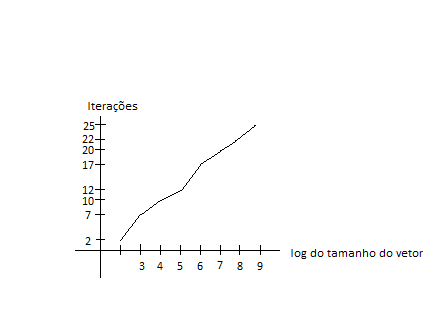
\includegraphics{plot-log.png} \\
    O gráfico está em escala exponencial em X, portanto ele dá a impressão que
cresce linearmente. Porém, na realidade, o crescimento é logarítmico.
        \item Esse algoritmo pode ser descrito utilizando dois algoritmos: um
de iteração ($\Theta(n)$) e outro de busca ($\Theta(logn)$). Segue abaixo uma
representação em pseudocódigo do algoritmo:
        \begin{algorithmic}[1]
            \Function{ExisteSoma}{S, x}
                \ForAll {$i \gets S$} \Comment{i é o índice, não o elemento}
                    \State {$ indiceComplemento \gets BuscaBinaria(S, S[i]-x) $}
                    \If {$ indiceComplemento \neq i $}
                        \State \Return{true}
                    \EndIf
                \EndFor
                \State \Return{false}
            \EndFunction
        \end{algorithmic}
        \item
            \begin{enumerate}
                \item Falso. Contra-exemplo: $O(n)$ é $O(n^2)$, mas $O(n^2)$ não é $O(n)$;
                \item Falso. Contra-exemplo: $\Theta(n) + \Theta(n^2) = \Theta(n^2)$;
                \item Verdadeiro. $g(n)$ domina assintoticamente $f(n)$, então $2^{g(n)}$ também domina $2^{f(n)}$;
                \item Falso. Considere $f(n) = n$ e $g(n) = n^2$. Não se pode afirmar que $g(n) = \Omega(n)$, pois $g(n)$ pode ser $\Omega(n^2)$.
            \end{enumerate}
\end{enumerate}

\begin{thebibliography}{1}
    \bibitem{thorup}
    M. Thorup, Undirected single-source shortest paths with positive integer
weights in linear time {\em JACM} {\bf 46} (1999).  \end{thebibliography}

\end{document}
